\ItemCategory{}
\ItemSubCategory{}
\ItemFolder{}

\chapter*{Staff of Chronurgy}\stepcounter{section}\phantomsection\addcontentsline{toc}{section}{Staff of Chronurgy}
\itemDescriptionAndImage{Wondrous Staff, Artifact (requires attunement by a Class-Lvl 3+ Wizard or Sorcerer)}{images/Magic_Items/Staff_of_Chronurgy.png}{6cm}\\

\begin{tikzpicture}[remember picture, overlay]%
	\node[xshift=0.55\columnwidth, yshift=-0.25\paperheight] at (current page.center) {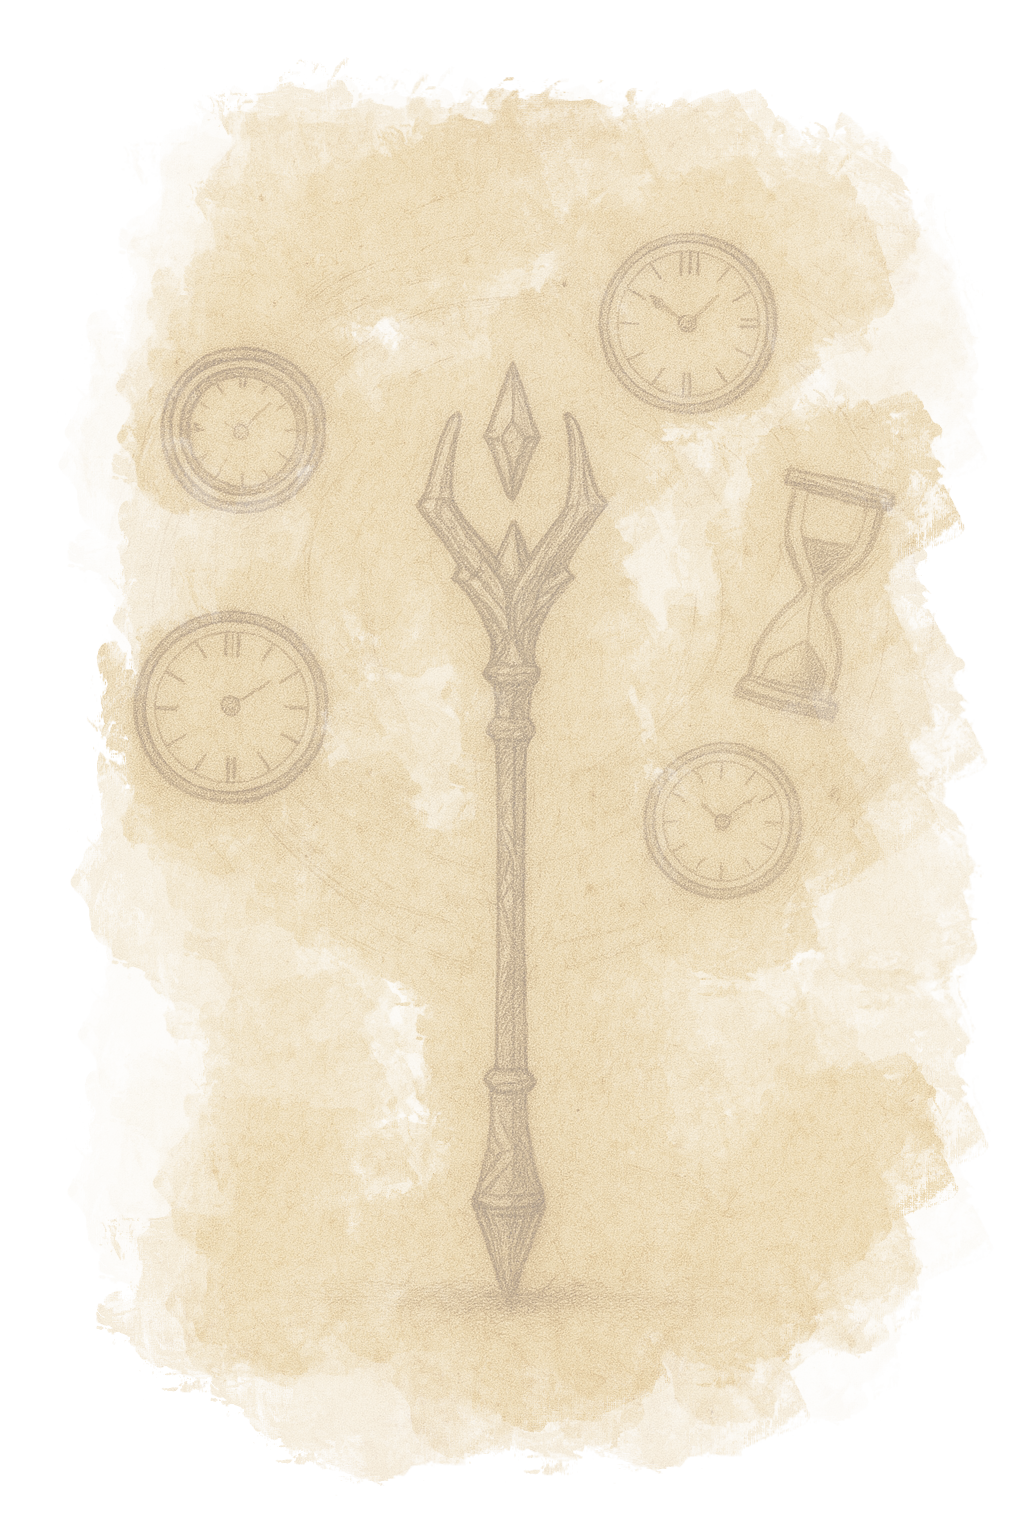
\includegraphics[width=1.1\columnwidth]{%
		images/Magic_Items/Staff_of_Chronurgy_background.png%
	}};%
\end{tikzpicture}%

\section*{Appearance}
{\entryfont The Staff of Chronurgy is a slender, elegant rod of dark metal inlaid with fine arcane etchings. Its shaft is straight and balanced, tapering to a pointed finial at the base. At the top, two curved prongs rise upward, holding aloft a small crystalline shard that floats, suspended by unseen magic. The shard glimmers faintly with shifting hues of blue and silver, as though reflecting the passage of time itself. Around the staff, subtle traces of arcane power manifest as fleeting images of clock faces and hourglasses, appearing and fading like echoes of time's flow.}
\section*{History}
{\entryfont Little is truly known of the Staff of Chronurgy. Scholars claim it has surfaced only rarely throughout history, always in times when the flow of time itself seemed unsettled. Some tales whisper that it was crafted by an archmage who sought to bind hours and moments as others bind steel and stone, while others insist it simply appeared in the hands of those fated to wield it. Records are fragmentary, and even chronomancers admit that its origins are shrouded in obscurity. What is known, however, is that wherever the staff emerges, the weave of time bends subtly around it - causing events, however small, to shift in unforeseen ways.}
\section*{Magic}
{\entryfont Unlike other arcane implements, it does not channel familiar schools of magic - instead, it awakens long-forgotten chronurgy spells, most of which remain undocumented and unstudied. Those who have witnessed its use describe moments unraveling, seconds looping back upon themselves, or entire actions erased from memory as though they never occurred.}
\vfill\eject
\subsection*{Gameplay Mechanics}
{\entryfont The Staff of Chronurgy holds a maximum number of charges equal to the value listed for each state. It regains expended charges as specified daily at dawn.
\subsubsection*{Dormant State}
\textbf{Charges: 3, Recharge: 1d2 + 1}
\begin{itemize}
	\item The wielder learns the Sapping Sting Cantrip. Intelligence is the spellcasting ability for this spell.
	\item While holding the staff, the wielder can expend some of its charges to cast one of the following spells from it, using their spell save DC and spellcasting ability and without requiring any Material component:
	\begin{itemize}
		\item Gift of Alacrity (1 Charge)
		\item Fortune's Favor (2 Charges)
	\end{itemize}
\end{itemize}
\subsubsection*{Awakened State}
\textbf{Charges: 5, Recharge: 1d4 + 1}
\begin{itemize}
	\item The wielder gains a +1 bonus to Spell Attacks and Spell Save DC.
	\item The following spells to the list of spells the staff may be used to cast are added:
	\begin{itemize}
		\item Wristpocket (2 Charges)
		\item Pulse Wave (3 Charges)
	\end{itemize}
	\item Once per Long Rest, when you cast a spell using a spell slot of 2nd level or lower, you can condense the spell into a mote (AC 15, HP 1, Immunity: Poison and Psychic) which manifests at the top of the staff. The spell itself is frozen in time at the moment of casting and held within the magical shard for 1 hour. When the duration ends, or if the mote is destroyed, it vanishes in a flash of light, and the spell is lost.
	
	A creature holding the shard can use its action to release the spell within, whereupon the shard disappears. The spell uses your spell attack bonus and save DC, and the spell treats the creature who released it as the caster for all other purposes.
\end{itemize}
\subsubsection*{Exalted State}
\textbf{Charges: 7, Recharge: 1d6 + 1}
\begin{itemize}
	\item The bonus to Spell Attacks and Spell Save DC increases to a +2.
	\item The following spells to the list of spells the staff may be used to cast are added:
	\begin{itemize}
		\item Temporal Shunt (5 Charges)
		\item Tether Essence (7 Charges)
	\end{itemize}
	\item The spell that can be stored within the mote can be one that used a spell slot of level 4 or lower.
\end{itemize}}
\vfill\eject
\DndSpellHeader
  {Sapping Sting}
  {Necromancy Cantrip}
  {Action}
  {30 Feet}
  {V, S}
  {Instantaneous}

\noindent You sap the vitality of one creature you can see in range. The target must succeed on a Constitution saving throw or take 1d4 necrotic damage and fall prone.

\subparagraph*{Cantrip Upgrade} The damage increases by one die when you reach levels 5 (2d4), 11 (3d4), and 17 (4d4).

\DndSpellHeader
  {Gift of Alacrity}
  {1st-Level Divination (Dunamancy: Chronurgy)}
  {1 Minute}
  {Touch}
  {V, S}
  {8 Hours}

\noindent You touch a willing creature. For the duration, the target can add 1d8 to its initiative rolls.

\DndSpellHeader
  {Fortune's Favor}
  {2nd-Level Divination (Dunamancy)}
  {1 Minute}
  {60 Feet}
  {V, S, M (a white pearl worth at least 100 gp, which the spell consumes)}
  {1 Hour}

\noindent You impart latent luck to yourself or one willing creature you can see within range. When the chosen creature makes an attack roll, an ability check, or a saving throw before the spell ends, it can dismiss this spell on itself to roll an additional d20 and choose which of the d20s to use. Alternatively, when an attack roll is made against the chosen creature, it can dismiss this spell on itself to roll a d20 and choose which of the d20s to use, the one it rolled or the one the attacker rolled.

If the original d20 roll has advantage or disadvantage, the creature rolls the additional d20 after advantage or disadvantage has been applied to the original roll.

\DndSpellHeader
  {Wristpocket}
  {2nd-Level Conjuration (Ritual) (Dunamancy)}
  {Action}
  {Self}
  {S}
  {Concentration, Up to 1 Hour}

\noindent You flick your wrist, causing one object in your hand to vanish. The object, which only you can be holding and can weigh no more than 5 pounds, is transported to an extradimensional space, where it remains for the duration.

Until the spell ends, you can use your action to summon the object to your free hand, and you can use your action to return the object to the extradimensional space. An object still in the pocket plane when the spell ends appears in your space, at your feet.

\DndSpellHeader
  {Pulse Wave}
  {3rd-Level Evocation (Dunamancy)}
  {Action}
  {Self (30-Foot Cone)}
  {V, S}
  {Instantaneous}

\noindent You create intense pressure, unleash it in a 30-foot cone, and decide whether the pressure pulls or pushes creatures and objects. Each creature in that cone must make a Constitution saving throw. A creature takes 6d6 force damage on a failed save, or half as much damage on a successful one. And every creature that fails the save is either pulled 15 feet toward you or pushed 15 feet away from you, depending on the choice you made for the spell.

In addition, unsecured objects that are completely within the cone are likewise pulled or pushed 15 feet.

\DndSpellHeader
  {Temporal Shunt}
  {5th-Level Transmutation (Dunamancy: Chronurgy)}
  {Reaction, taken when a creature you see makes an attack roll or starts to cast a spell}
  {120 Feet}
  {V, S}
  {1 Round}

\noindent You target the triggering creature, which must succeed on a Wisdom saving throw or vanish, being thrown to another point in time and causing the attack to miss or the spell to be wasted. At the start of its next turn, the target reappears where it was or in the closest unoccupied space. The target doesn't remember you casting the spell or being affected by it.

\DndSpellHeader
  {Tether Essence}
  {7th-Level Necromancy (Dunamancy)}
  {Action}
  {60 Feet}
  {V, S, M (a spool of platinum cord worth at least 250 gp, which the spell consumes)}
  {Concentration, Up to 1 Hour}

\noindent Two creatures you can see within range must make a Constitution saving throw, with disadvantage if they are within 30 feet of each other. Either creature can willingly fail the save. If either save succeeds, the spell has no effect. If both saves fail, the creatures are magically linked for the duration, regardless of the distance between them. When damage is dealt to one of them, the same damage is dealt to the other one. If hit points are restored to one of them, the same number of hit points are restored to the other one. If either of the tethered creatures is reduced to 0 hit points, the spell ends on both. If the spell ends on one creature, it ends on both.